\chapter{Conception and Design}
In this chapter, the main parts of this program will be discussed, and the design will be explained.\\
The main idea of this program is to take a specific list of modules, and after some operations on them to ensure their validity, it should start to install the modules on VirtualBox\cite{virtualbox}.\\
Installing the modules and transferring files is done through SSH, which means realistically, that SSH module must always be present or rather be installed first for other modules to function.

\section{Modules}
A module is a user-defined package, that does one or more sets of tasks and it has 3 main components that allow it to be automated:
\begin{enumerate}
    \item \textbf{Metadata}
    \item \textbf{Main script}
    \item \textbf{Resources}
\end{enumerate}
The metadata is a configuration file written in YAML, it defines all of the features of the corresponding module, and especially the provided and/or the needed dependencies. This file can also hold important configurations which are essential for the functionality of the module.
Metadata has some rules that will be covered later in this chapter.

The main script is a Bash script, which acts as a start point to the module, it usually has the initial SSH connecting and resources copying commands.

Resources are everything else that the module needs to perform its intended task. For example, it can be website static files, SQL dumps, or other helper scripts.
\\
\begin{figure}[!ht]
\centering
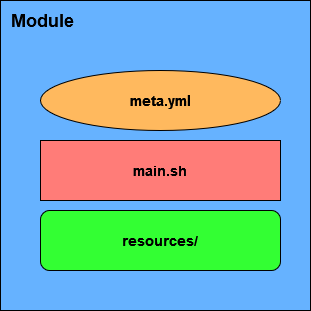
\includegraphics[width=0.5\textwidth]{resources/figures/module.png}
\caption{Module's content}
\end{figure}

\section{Process}
There are two considered ways to achieve the process to automate the install of modules:
First by implementing a bash script that serves as an entry point to all modules, and then sending commands with a python script to it.\\

\begin{figure}[!ht]
\centering
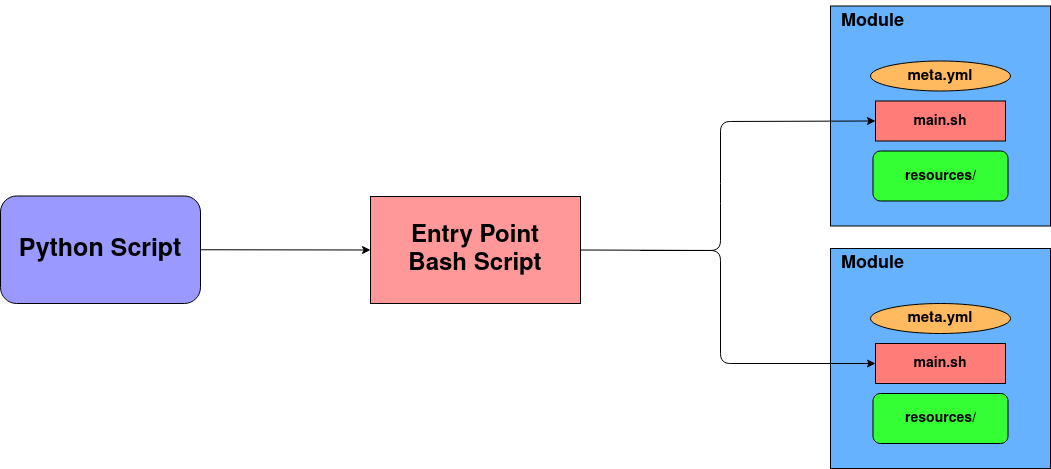
\includegraphics[width=0.95\textwidth]{resources/figures/process1.png}
\caption{Process design 1}
\label{fig:process1}
\end{figure}

\clearpage

The second way is by controlling the modules from the main python script itself, this means that this python script is responsible for orchestrating the execution of bash scripts inside the modules.\\

\begin{figure}[!ht]
\centering
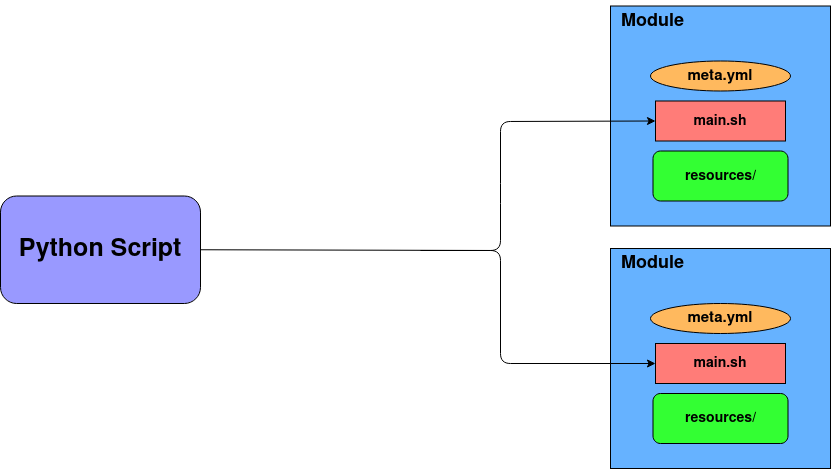
\includegraphics[width=0.95\textwidth]{resources/figures/process2.png}
\caption{Process design 2}
\label{fig:process2}
\end{figure}

However, before the main python script executes the bash scripts in the modules, there need to be some necessary operations done.\\
First of all, metadata must be validated to ensure proper parsing of the YAML file, and afterward, the configurations available in the metadata must be parsed and then replaced with placeholders in the module’s scripts.\\
The intended designed process will then look like the following figure \ref{fig:allprocess}:\\
\\

\begin{figure}[!ht]
\centering
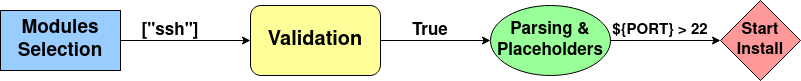
\includegraphics[width=0.95\textwidth]{resources/figures/allprocess.png}
\caption{Full process}
\label{fig:allprocess}
\end{figure}

\clearpage

\section{Validation}
To ensure the success of the installation process, the metadata of the modules needs to be validated. A set of rules were declared to help creators of modules write a valid metadata file, this set of rules are written in a form of schema.\\
Furthermore, with the help of python package “cerberus”\cite{cerberus}, this schema is validated against the metadata YAML file. In case of unsuccessful validation, the installing process will not begin.\\
These designed rules are explained in the following pseudo-code:

\begin{lstlisting}[caption=YAML Schema, style=pythonstyle]
name:
provides:
    tech:  # list
      - entry:  # map
          name:  # string
          version:  # string
          config:  # list
    tech-config:
      - entry:
          name:
          version:
          config:
needs:
    tech:
      - entry:
          name:
          version:
          config:
\end{lstlisting}

Each module has a “name” entity and provides one or more sets of dependencies and configurations. Entries under “tech” are the dependencies that this module provides. Lastly, the entries under “tech-config” are the configurations this module provides without providing the corresponding dependency for it.\\
Every “tech” entry has the name of dependency, the version of it, and all configurations it supplies. Same structure is for “tech-config”.\\
For every configuration, the “name”, “file”, and “value” are listed.
\begin{enumerate}
  \item \textbf{“name”} is the name of the placeholder that the parser will be replacing.
  \item \textbf{“file”} is the name of the file, in which the placeholder should be replaced
  \item \textbf{“value”} is a list of values that will be replacing the placeholder
\end{enumerate}

\begin{lstlisting}[caption=YAML Schema, style=pythonstyle]
config:  # list
    - name:  # string
      file:  # string
      value:  # list
\end{lstlisting}
It could be noticed, that the “needs” entity does not have a “tech-config” entity of its own. That is for the reason that a module can not need a certain configuration without needing its dependency as well, thus deprecating the use of “tech-config” for it.


\section{Template Engine} \label{temp_engine}
The metadata defines what dependencies the module has, and what configuration it provides and/or needs. This shows that parsing the metadata file must be done in an organized way.

When a module has a configuration, it consists of a placeholder in the main bash script or any other scripts in the resources folder. These placeholders are the locations where the values from the metadata should be replaced. This is where a template engine is used.

“A template engine enables you to use static template files in your application. At runtime, the template engine replaces variables in a template file with actual values, and transforms the template into an HTML file sent to the client.”\cite{template}

This can be done by using an internal package of python called “string”, this package has a helpful function, namely “Template”\cite{string}. It replaces placeholders with identifiers of the form \$\{PLACEHOLDER\}.
